\documentclass{standalone}
\usepackage{tikz}
\definecolor{C1}{RGB}{73,0,146}
\usepackage{ifthen}
\newcommand{\myaxis}[7][help lines]{%[formatting of lines]{xlabel}{xleft}{xright}{ylabel}{yleft}{yright}
	\ifthenelse{\lengthtest{#3 pt=0 pt}}{}{
		\draw[ <-,#1] (-#3,0)--(0,0);
		}
	\ifthenelse{\lengthtest{#4 pt=0 pt}}{
		\draw[#1] (0,0)node[right]{$#2$};}{
		\draw[ ->,#1] (0,0)--(#4,0)node[right]{$#2$};
		}
	\ifthenelse{\lengthtest{#6 pt= 0 pt}}{
		}{
		\draw[ <-,#1] (0,-#6)--(0,0);}
	\ifthenelse{\lengthtest{#7 pt= 0 pt}}{
		\draw[#1] (0,0)node[above]{$#5$};
		}{
		\draw[ ->,#1] (0,0)--(0,#7)node[above]{$#5$};}
}

\begin{document}
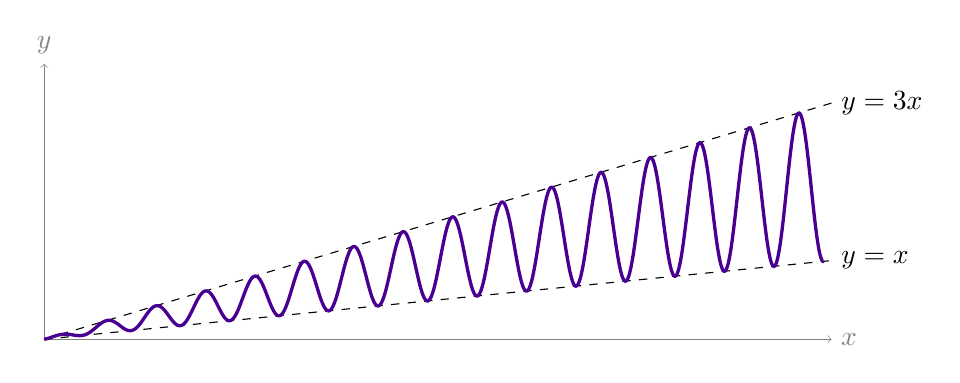
\begin{tikzpicture}
\myaxis{x}{0}{10}{y}{0}{3.5};
\draw[dashed] (0,0)--(10,1)node[right]{$y=x$};
\draw[dashed] (0,0)--(10,3)node[right]{$y=3x$};
\draw[C1, very thick] plot[domain=0:99,smooth,samples=10000,xscale=0.1,yscale=0.01](\x,{\x*(sin(\x r)+2)});

\end{tikzpicture}

\end{document}